% !TEX root = ../my-thesis.tex
%
\chapter{Appendix}
\label{sec:appendix}
\section{Probability Distributions}
\subsection{The Normal Distribution}
The normal distribution is an important type of continuous probability distribution in stochastics. The special significance of the normal distribution is based, among other things, on the central limit theorem, according to which distributions that result from the additive combination of a large number of independent influences are approximately normally distributed under weak conditions. \\
The density is given by
\begin{equation}
    f\left(x|\mu,\sigma\right)=\frac{1}{\sigma\sqrt{2\pi}}\exp\left(-\frac{1}{2}\left(\frac{x-\mu}{\sigma}\right)^2\right).
\end{equation}
The first two moments of the distribution are given by
\begin{align}
    \mathbb{E}\left[X\right] &= \mu \\
    \hbox{Var}\left[X\right] &= \sigma^2.
\end{align}
The graph of this density function has a "bell-shaped form" and is symmetrical with $\mu$ as the centre of symmetry \autocite[][83-85]{fahrmeir2016statistik}.
\subsection{The Poisson Distribution}
The Poisson distribution is a discrete probability distribution that can be used to model the number of events that occur independently of each other at a constant mean rate in a fixed time interval or spatial area. \\
The density is given by
\begin{equation}
    f\left(k\right)=\mathbb{P}\left(X=k\right)=\begin{cases}
    \frac{\lambda^k}{k!}\exp\left(-\lambda\right) & \hbox{for }x\in\left\lbrace0,1,...\right\rbrace \\
    0 & \hbox{else}
    \end{cases}
\end{equation}
with $\lambda$ representing the expected value of $X$.  \\
The first two moments of the distribution are given by
\begin{align}
    \mathbb{E}\left[X\right] &= \lambda \\
    \hbox{Var}\left[X\right] &= \lambda.
\end{align}
For $\lambda\geq10$ the distribution becomes approximately symmetrical and can thus be approximated by a normal distribution \autocite[][243]{fahrmeir2016statistik}.
\subsection{The Negative Binomial Distribution}
The negative binomial distribution is a univariate probability distribution that belongs to the discrete probability distributions. It models the number of trials required to achieve a given number of successes in a Bernoulli process. \\
The density is given by
\begin{equation}
    f\left(k,r,p\right)=\mathbb{P}\left(X=k\right)=\begin{pmatrix} k+r-1\\r-1\end{pmatrix}\left(1-p\right)^kp^r,
\end{equation}
with $r$ the number of successes, $k$ the number of failures, and $p$ the probability of success. \\
The first two moments of the distribution are given by
\begin{align}
    \mathbb{E}\left[X\right] &= \frac{pr}{1-p} \\
    \hbox{Var}\left[X\right] &= \frac{pr}{\left(1-p\right)^2}.
\end{align} 
For large values of $r$, the negative binomial distribution can be approximated by a normal distribution
\cite{haldane1941fitting}.
\clearpage
\section{Distribution Fits}
\subsection{Distribution Fits for Germany}
% \begin{figure}[H]
%     \centering
%     \includesvg[width = 0.8\textwidth]{fit_normal_germany.svg}
%     \caption{A normal fit to the number of cases in German municipalities}
%     \label{fitNormalGermany}
% \end{figure}
\begin{figure}[H]
    \centering
    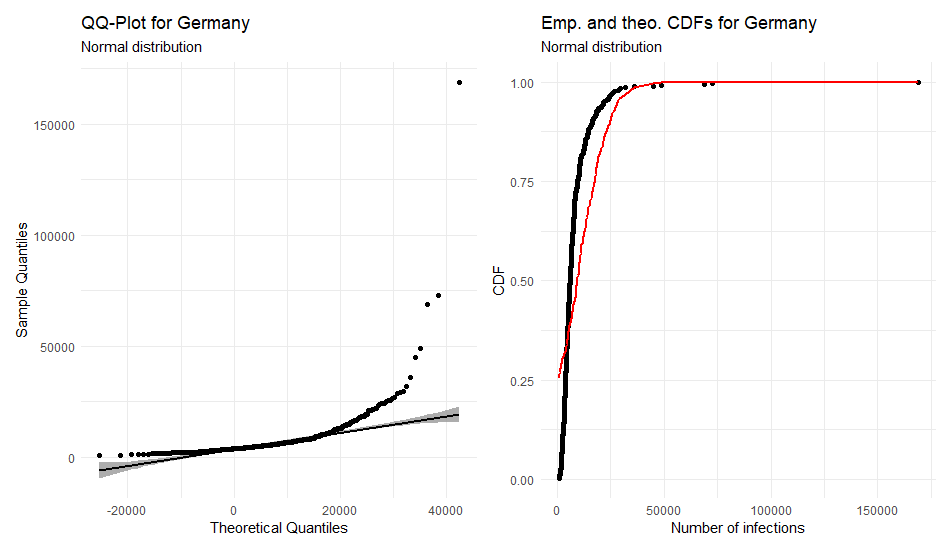
\includegraphics[width = 0.8\textwidth]{fit_normal_germany.png}
    \caption{A normal fit to the number of cases in German municipalities}
    \label{fitNormalGermany}
\end{figure}
% \begin{figure}[H]
%     \centering
%     \includesvg[width = 0.8\textwidth]{fit_poisson_germany.svg}
%     \caption{A Poisson fit to the number of cases in German municipalities}
%     \label{fitPoissonGermany}
% \end{figure}
\begin{figure}[H]
    \centering
    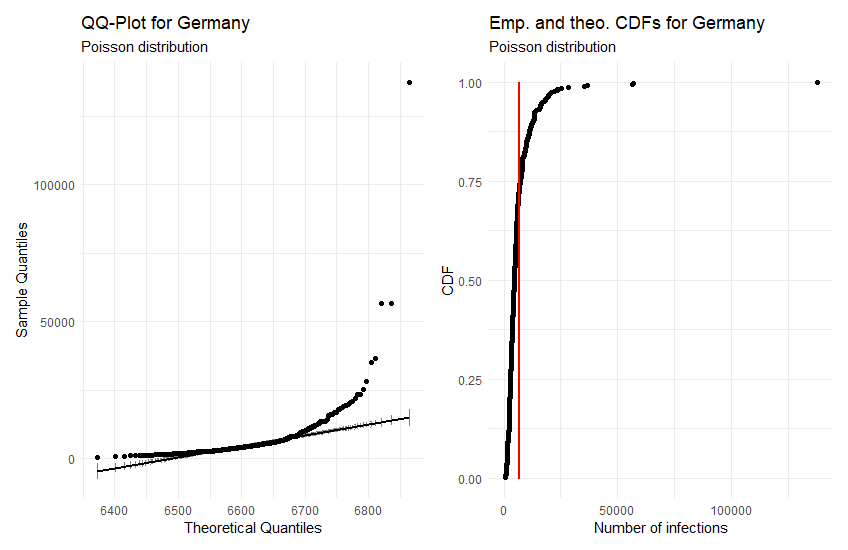
\includegraphics[width = 0.8\textwidth]{fit_poisson_germany.png}
    \caption{A Poisson fit to the number of cases in German municipalities}
    \label{fitPoissonGermany}
\end{figure}
\subsection{Distribution Fits for Norway}
% \begin{figure}[H]
%     \centering
%     \includesvg[width = 0.8\textwidth]{fit_normal_norway.svg}
%     \caption{A normal fit to the number of cases in Norwegian municipalities}
%     \label{fitNormalNorway
% \end{figure}
\begin{figure}[H]
    \centering
    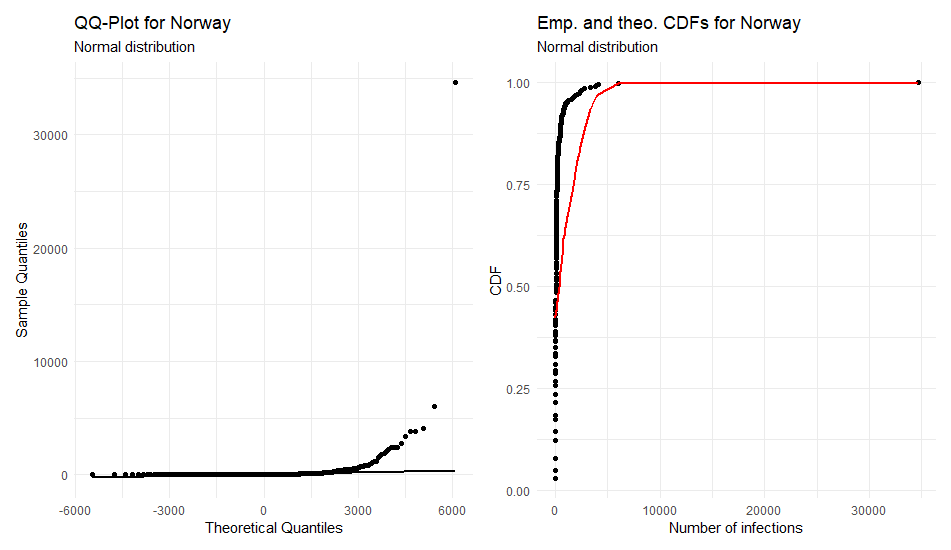
\includegraphics[width = 0.8\textwidth]{fit_normal_norway.png}
    \caption{A normal fit to the number of cases in Norwegian municipalities}
    \label{fitNormalNorway}
\end{figure}
% \begin{figure}[H]
%     \centering
%     \includesvg[width = 0.8\textwidth]{fit_poisson_norway.svg}
%     \caption{A Poisson fit to the number of cases in Norwegian municipalities}
%     \label{fitPoissonNorway}
% \end{figure}
\begin{figure}[H]
    \centering
    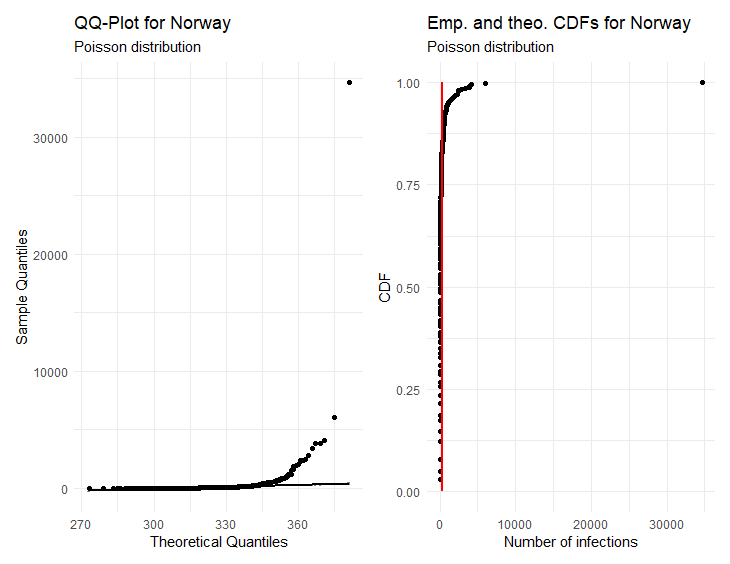
\includegraphics[width = 0.8\textwidth]{fit_poisson_norway.png}
    \caption{A Poisson fit to the number of cases in Norwegian municipalities}
    \label{fitPoissonNorway}
\end{figure}
\clearpage
\section{Code examples}
\subsection{Specifying the Different Types of Models}
\begin{lstlisting}[caption={Specifying different models in INLA.}, label={codeModels}, language=R]
# set the seed
set.seed(420)
# draw a sample
test <- sample(
    seq_len(nrow(newest_numbers)),
    size = floor(0.2 * nrow(newest_numbers))
  )
# get the number of infections for the test data
test_value <- newest_numbers$value[test]
# set the number of infections to NA in the train data
newest_numbers$value[test] <- NA
# define the link function
link <- rep(NA, nrow(newest_numbers))
link[which(is.na(newest_numbers$value))] <- 1
# define the penalised prior
prior_1 <- list(
  prec = list(
    prior = "pc.prec",
    param = c(1, 0.01)
  )
)
# create the neighbordhood matrix
nb <- poly2nb(newest_numbers)
# save the matrix
nb2INLA("maps/map.adj", nb)
g <- inla.read.graph(filename = "maps/map.adj")
# define the C matrix for the Leroux model
Q <- Diagonal(x = sapply(nb, length))
for (i in 2:nrow(newest_numbers)) {
  Q[i - 1, i] <- -1
  Q[i, i - 1] <- -1
}

C <- Diagonal(x = 1, n = nrow(newest_numbers)) - Q
# define the formula for besags proper model
formula_besag <- value ~
  pop_dens + urb_dens + sex +
  f(idarea_1, model = "besagproper", graph = g, hyper = prior_1)
# define the formula for bym2 model
formula_bym2 <- value ~
  pop_dens + urb_dens + sex +
  f(
    idarea_1, model = "bym2", graph = g,
    scale.model = TRUE, hyper = prior_1
  )
# define the formula for leroux model
formula_leroux <- value ~
  pop_dens + urb_dens + sex +
  f(idarea_1, model = "generic1", Cmatrix = C, hyper = prior_1)
# compute the models
res_besag <- inla(
  formula_besag,
  family = "nbinomial",
  data = newest_numbers,
  E = expected_count,
  control.predictor = list(
    compute = TRUE,
    link = link
  ),
  Ntrials = newest_numbers$population,
  control.compute = list(dic = TRUE, waic = TRUE, cpo = TRUE)
)
res_bym2 <- inla(
  formula_bym2,
  family = "nbinomial",
  data = newest_numbers,
  E = expected_count,
  control.predictor = list(
    compute = TRUE,
    link = link
  ),
  Ntrials = newest_numbers$population,
  control.compute = list(dic = TRUE, waic = TRUE, cpo = TRUE)
)
res_leroux <- inla(
  formula_leroux,
  family = "nbinomial",
  data = newest_numbers,
  E = expected_count,
  control.predictor = list(
    compute = TRUE,
    link = link
  ),
  Ntrials = newest_numbers$population,
  control.compute = list(dic = TRUE, waic = TRUE, cpo = TRUE)
)
\end{lstlisting}
\subsection{Making Predictions for the Test Data}
\begin{lstlisting}[caption={The code for making predictions in INLA.}, label={codePrediction}, language=R]
# create a vector to save the predictions to
predicted <- c()
# now make the predictions
for(i in seq_len(nrow(newest_numbers))) {
  predicted[i] <- inla.emarginal(
    function(x) x * newest_numbers$population[i],
    res_bym2$marginals.fitted.values[[i]]
  )
}
# calculate the MAE for the test data
mean(abs(predicted[test] - test))

\end{lstlisting}
\subsection{Variable Selection using INLA}
\begin{lstlisting}[caption={The code for variable selection in INLA.}, label={codeSelection}, language=R]
# define the stack
stack_all <- inla.stack(
  data = list(value = newest_numbers$value),
  A = list(1),
  effects = list(
    data.frame(
      Intercept = 1,
      newest_numbers[, c(2:15, 20:35, 43:46)]
    )
  )
)
# run backwards varaible selection
result_all_backwards <- INLAstep(
  fam1 = "nbinomial",
  newest_numbers,
  in_stack = stack_all,
  invariant = "Intercept",
  direction = "backwards",
  include = c(2:15, 20:35, 43:46),
  y = "value",
  y2 = "value",
  powerl = 1,
  inter = 1,
  thresh = 2,
  num.threads = 7
)
# run forwards variable selection
result_all_forwards <- INLAstep(
  fam1 = "nbinomial",
  newest_numbers,
  in_stack = stack_all,
  invariant = "Intercept",
  direction = "forwards",
  include = c(2:15, 20:35, 43:46),
  y = "value",
  y2 = "value",
  powerl = 1,
  inter = 1,
  thresh = 2,
  num.threads = 7
)
\end{lstlisting}
\subsection{Calculating the Posterior Mean}
\begin{lstlisting}[caption={Calculating the posterior mean of a coefficent.}, label={codePosteriorMean}, language=R]
inla.emarginal(exp, model_leroux$marginals.fixed$trade_tax)
# calculate the increase in risk for an increase 
# by 2 in the trade tax
inla.emarginal(
  exp,
  model_leroux$marginals.fixed$trade_tax
  ) ^ 2
\end{lstlisting}
\subsection{Calculating a Credibility Interval}
\begin{lstlisting}[caption={Extracting the credibility interval for a coefficient}, label={codeCredibility}, language=R]
inla.qmarginal(
  c(0.025,0.975),
  inla.tmarginal(
    exp,
    model_leroux$marginals.fixed$trade_tax
  )
)
\end{lstlisting}
\subsection{Best Spatial Models For Germany}
\subsubsection{Best Spatial Model using Demographic Variables}
\begin{lstlisting}[caption={The code for the demographic model.}, label={codeDemoGermany}, language=R]
prior_2 <- list(
  prec = list(
    prior = "pc.prec",
    param = c(0.5 / 0.31, 0.01)
  )
)
formula <- value ~
  Union + SPD + Gruene + FDP +
  die_linke + afd + 
  f(idarea_1, model = "generic1", Cmatrix = C, hyper = prior_2)
\end{lstlisting}
\subsubsection{Best Spatial Model using Infrastructural Variables}
\begin{lstlisting}[caption={The code for the infrastructure model.}, label={codeInfraGermany}, language=R]
prior_1 <- list(
  prec = list(
    prior = "pc.prec",
    param = c(1, 0.01)
  )
)
formula <- value ~
  marketplace + entertainment + sport + clinic +
  hairdresser + shops + place_of_worship + retail + nursing_home +
  restaurant + aerodrome + office + platform + schools +
  higher_education + kindergarten + bakeries + 
  f(
    idarea_1, model = "bym2", graph = G,
    scale.model = TRUE, hyper = prior_1
  )
\end{lstlisting}
\subsubsection{Best Spatial Model using Both Types of Variables}
\begin{lstlisting}[caption={The code for the demographic + infrastructure model.}, label={codeBothGermany}, language=R]
prior_1 <- list(
  prec = list(
    prior = "pc.prec",
    param = c(1, 0.01)
  )
)
formula <- value ~
  schools + afd + die_linke + pop_dens +
  place_of_worship + entertainment + bakeries + SPD +
  platform + sport + nursing_home + welfare_recipients +
  FDP + kindergarten + log(trade_tax) + office +
  f(
    idarea_1, model = "bym2", graph = g,
    scale.model = TRUE, hyper = prior_1
  )
\end{lstlisting}
\subsection{Best Spatial Models For Norway}
\subsubsection{Best Spatial Model using Demographic Variables}
\begin{lstlisting}[caption={The code for the demographic model.}, label={codeDemoNorway}, language = R]
prior_1 <- list(
  prec = list(
    prior = "pc.prec",
    param = c(1, 0.01)
  )
)
formula <- value ~
  unemp_immg + unemp_tot
  f(
    idarea_1, model = "generic1",
    Cmatrix = C, hyper = prior_1
  )
\end{lstlisting}
\subsubsection{Best Spatial Model using Infrastructural Variables}
\begin{lstlisting}[caption={The code for the infrastructural model.}, label={codeInfraNorway}, language = R]
prior_1 <- list(
  prec = list(
    prior = "pc.prec",
    param = c(1, 0.01)
  )
)
formula <- value ~
  schools + shops + place_of_worship + office +
  schools + nursing_home + kindergarten + restaurant +
  f(
    idarea_1, model = "besagproper",
    graph = g, hyper = prior_1
  )
\end{lstlisting}
\subsubsection{Best Spatial Model using Both Types of Variables}
\begin{lstlisting}[caption={The code for the demographic + infrastructure model.}, label={codeBothNorway}, language=R]
prior_1 <- list(
  prec = list(
    prior = "pc.prec",
    param = c(0.5 / 0.31, 0.01)
  )
)
formula <- value ~
  schools + unemp_tot + restaurant + sex + 
  median_age + pop_dens + construction_pt_work +
  workers_ft_work + higher_education + clinic +
  f(
    idarea_1, model = "besagproper",
    graph = g, hyper = prior_2
  )
\end{lstlisting}
\clearpage